\documentclass[12pt,letterpaper]{article}
\usepackage{pdfpages}
\usepackage{fancyhdr}
\usepackage[colorlinks=true, urlcolor=blue, linkcolor=blue]{hyperref}
\usepackage{graphicx}
\usepackage[top=1.4in, left=0.5in, right=0.5in, bottom=0.8in]{geometry}
\usepackage[T1]{fontenc}
\usepackage{helvet}
\pagestyle{fancy}
\renewcommand{\headrulewidth}{0pt}
\renewcommand{\footrulewidth}{0pt}
\setlength{\parindent}{0em}
\setlength{\parskip}{1em}


\fancyfoot[C]{\setlength{\unitlength}{1in}\begin{picture}(5,0)\put(-1.8,-1){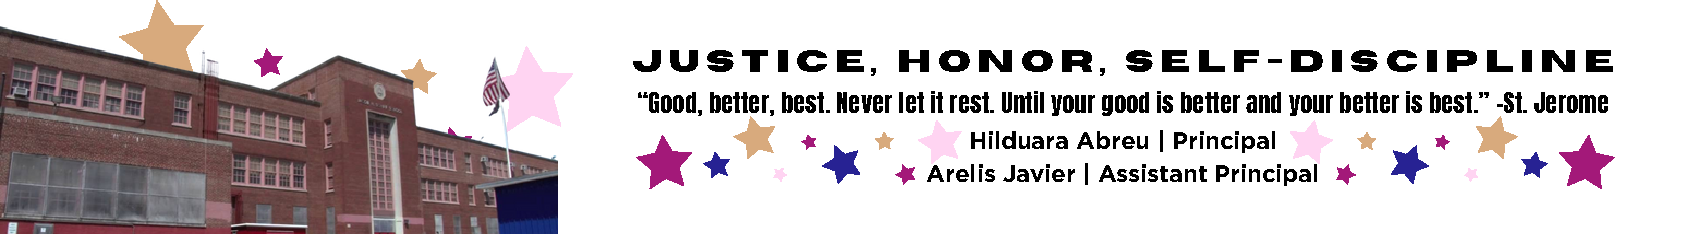
\includegraphics[width=8.8in,height=1.3in]{logo-1}}\end{picture}}
\fancyhead[C]{\setlength{\unitlength}{1in}\begin{picture}(5,0)\put(-1.9,-1){
\includegraphics[width=8.9in,height=1.3in]{logo-2}}\end{picture}}

\pagenumbering{gobble}
\addtolength{\evensidemargin}{-2in}
\addtolength{\topmargin}{-0.5in}
\addtolength{\textwidth}{0in}
%%%%%%%%%%%%%%%%%%%%%%%%%%%%%%%%%%%%%%%%%%%%%%%%%%%%%%%%%%%%%%%%%%

\begin{document}
\vspace*{0.5in}
School Website: \href{https://www.ps192.org}{www.ps192.org}

\textbf{Principal's Message May 2024}

Dear Parents and Guardians,

As we welcome the pleasant change in weather, we are excited to announce several upcoming events and
important dates at our school:
\begin{itemize}
\item NYSESLAT Testing: For all bilingual students and ELLs in monolingual classes (Grades K-5) from
May 7th to May 24th, 2024.
\item New York State Math Test: Scheduled for May 7th to May 10th, 2024.
\item Parent-Teacher Conferences: Please join us on Thursday, May 9th, 2024, from 4:30 PM to 7:30 PM.
\item Teacher Appreciation Week: We will honor our staff with a luncheon on Thursday, May 9th, 2024, and invite all parents to a special breakfast on Friday, May 10th, 2024, at 8:00 AM in the gymnasium.
\item New York State Science Performance Test: Taking place from May 15th to May 16th, 2024.
\item United at The Palace: Scheduled for May 17th, 2024, at 5:00 PM.
\end{itemize} 
We aim for the Parent-Teacher Conferences to be a productive time for collaboration between parents and
teachers, fostering an environment where our students can excel and meet their full potential. We look
\pagebreak
\vspace*{0.7in}
forward to enjoying the spring season together and seeing you at the various workshops and school
events planned. Thank you for your continual support, and a very Happy Mother’s Day to all celebrating!

Warm regards, 


\includegraphics[width=0.12\textwidth]{hil_signature}

\textbf{Hilduara Abreu}

\textbf{Principal P.S. 192}

\textit{The School of Joyful Learning!}
\pagebreak
\vspace*{0.7in}

School Website: \href{https://www.ps192.org}{www.ps192.org}

\textbf{Mensaje de la directora mayo de 2024}

Queridos padres y guardianes,

Mientras damos la bienvenida al agradable cambio de clima, nos complace anunciar varios eventos y fechas importantes en nuestra escuela:
\begin{itemize}
\item Pruebas NYSESLAT: Para todos los estudiantes bilingües y ELL en clases monolingües (grados K-5) desde 7 de mayo al 24 de mayo de 2024.
\item Pruebas NYSESLAT: Para todos los estudiantes bilingües y ELL en clases monolingües (grados K-5) desde 7 de mayo al 24 de mayo de 2024.
\item Prueba de matemáticas del estado de Nueva York: programada para el 7 al 10 de mayo de 2024.
\item Conferencias de padres y maestros: únase a nosotros el jueves 9 de mayo de 2024, de 4:30 p. m. a 7:30 p. m.
\item Semana de Agradecimiento a los Maestros: Honraremos a nuestro personal con un almuerzo el jueves 9 de mayo de 2024 e invitar a todos los padres a un desayuno especial el viernes 10 de mayo de 2024 a las 8:00 a.m. en el gimnasio.
\item Prueba de rendimiento en ciencias del estado de Nueva York: se llevará a cabo del 15 al 16 de mayo de 2024.
\item Unidos en EL Palace: Programado para el 17 de mayo de 2024, a las 5:00 p.m.
\end{itemize}

Nuestro objetivo es que las conferencias de padres y maestros sean un momento productivo para la colaboración entre padres y maestros, fomentando un ambiente donde nuestros estudiantes puedan
\pagebreak
\vspace*{0.7in}
sobresalir y alcanzar su máximo potencial. Esperamos disfrutar juntos de la temporada de primavera y verlos en los distintos talleres y eventos escolares. ¡Gracias por su continuo apoyo y un muy feliz Día de la Madre a todos los que celebran!

Un cordial saludo,


\includegraphics[width=0.2\textwidth]{hil_signature}

\textbf{Hilduara Abreu}

\textbf{Principal P.S. 192}

\textit{La escuela donde el aprendizaje es divertido!}

\end{document}







